% Chapter1
\chapter{Introduction} \label{chapter:introduction} 
\section{General}
 Today everybody can create an App for any Platform. In this world, most of the pupils use Smartphones. So in that case this work describes from which modules or elements  the App NAVAR is created of.  Furthermore it shows how to use the Modules in General and how to deploy them. However for this project we used three programing languages. For the user Interface we used JQuery Mobile Framework. This Application has been developed for the Android platform.  We wrote this application in Android because the client recommended it. The SDK  for the Tracking system is implemented  in this app and it is developed for Android and IOS.   
 \\\\
 The following point is, that the project uses Javascript,HTML5 ,CSS  and the Framework JQuery Mobile for the user interface. The main problem was to combine the user interface with the tracking logic implementation. Further more the connection between the smartphone and the Navision Server was not so easy to implement.
 In this chapter it describes the programing languages and the Framework, that was have used for this project:
 \begin{enumerate}
 \item Java
 \item JavaScript,HTML5,CSS
 \item jQuery Mobile
 \item C\#
 \end{enumerate}
 \newpage
 \section{Augmented Reality}
 \subsection{What is Augmented Reality ?}
  Augmented Reality(AR) is a type of  virtual environment. It aim to duplicate the world's environment into the computer. The idea of AR is, it combines the scene of the real world with virtual scene generated by the device. Furthermore the virtual scene augments the scene with additional Information. So the virtual scene which is designed to enhance the users sensory perception of the virtual World, they are seeing or interacting with. The virtual scenes which are generated by computer are sensory inputs such as sounds, videos, graphics or GPS data. It replaces real world with a simulated one.\cite{augmenteddef}
 \\\\
 A good example for Augmented Reality are the sport games which will be live broadcasted. On the TV you can see the scores or other information. This shows that,  Augmentation is conventionally in real-time and in semantic context with environmental elements. The advanced AR technology helps to surround the real world of the user with information, so it becomes interactive and digitally manipulable.\cite{augmenteddef}
 \\
 \subsection{Augmented reality vs Virtual Reality}
 
 \textit{'Augmented reality (AR) and virtual reality (VR) are fields in which the lines of
 distinction are kind of blurred. To put it another way, you can think of VR as the
 precursor to AR, with some parts overlapping in both. The main difference
 between the two technologies is that VR does not use a camera feed. All the
 things displayed in VR are either animations or prerecorded bits of film.
 '\cite{AugmentedBook}}
 \subsection{Companies for Augmented Reality}
 There are three major Companies, which produce Software or programs to use the Augmented Reality Technology for smart phones or Google Glasses.  The name of the first company is Metaio GmbH. It is a German corporation. This company was founded in 2003. It offers Augmented Reality for industrial and automotive sectors for product design and factory planning. This concern already created few Apps for Smartphones. They are working with other companies together to create Applications for mobile phones, such as an app for an E-manual for  Audi. This app  starts the camera of the mobile device and scans the car components, such as the steering of the car. Then it tells the user which functionality the steering has. Furthermore the firm is very young and with this technology it has a big developmental push. It has a big development platform for creating applications with AR. So it sells products such as SDKs and other programs to create our own AR Applications for smartphones and Desktop PCs.
 \\
 \\
 The second Company is a spin-off company from the Swiss Federal Institute of Technology(ETH) in Zurich and the name of  the product is Kooaba. It was founded  in November 2006 . The mission of this product is to unlock the information which has been captured in images in using the sophisticated image recognition technology. This firm is a competitor to Metaio GmbH.
 \\
 \\ 
 The last popular company is Google. They created the Google glasses and another project called tango.  For the project tango they created a specified mobile phone with two back cameras..
 \\
 \\
 
 \textit{ Project Tango is an attempt to create a mobile device unlike like any other, a mobile device that shares our sense of space and movement, that understands and perceives the world the same way we do.\cite{Tango}}
 \\
 \\
 \textit{
 They have been collaborating with universities, research labs, and industrial partners who share this passion spanning 9 countries around the world to concentrate the past 10 years of research in robotics and computer vision into a unique mobile phone. We now have prototypes ready to put into the hands of eager development partners that can help us imagine the possibilities and to transform those ideas into reality.\cite{Tango}
 }
 \\
 \\
 Augmented Reality is used by Smartphones and Google Glasses. Google glasses is a very good product for the AR Technology
 \begin{figure}[htbp]
 \centering
 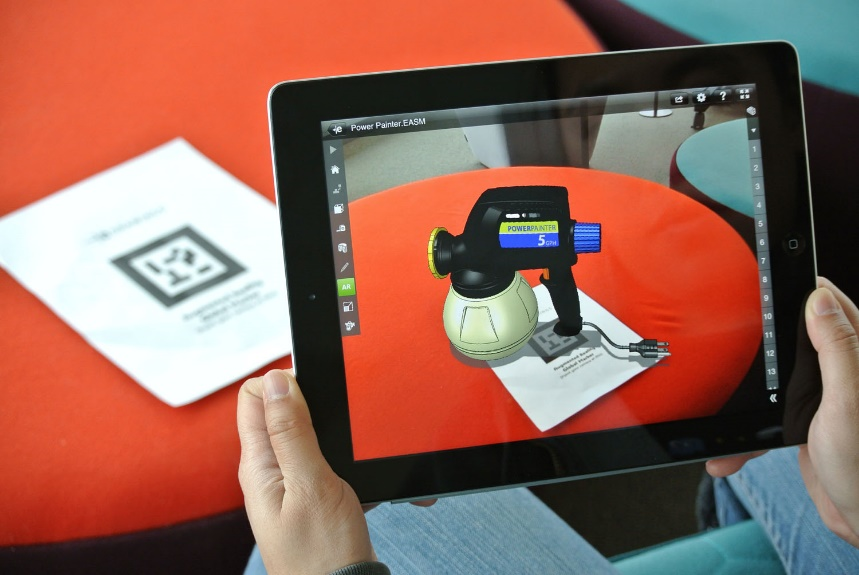
\includegraphics[width=240pt,height=180pt,keepaspectratio]{graphics/ARpad.png}
 \caption{\cite{ARpad}}
 \end{figure}
 [4]\\
 \\
 \subsection{Google Glasses}
 The new innovation from google was really exciting. Google glass is a new gadget for the whole world. Furthermore it combines the reality with virtual components . This projects launch event was in 2012 .Google Glass is the name for a type of wearable computer. It was created by the Google's Project team Glass. It provides Augmented Reality for users by visually connecting them to an Android-run heads up display that offers many of the features of an Android smartphone. With this device the user can connect to Google's key cloud features such as maps, calendar ,Gmail, Google+ and Google Places. Google hopes to have the gadget in the market in the near future. So they expect the technology to cost about as much as a smartphone.\cite{glasses01}
 \\
 \\
 \begin{figure}[htbp]
 \centering
 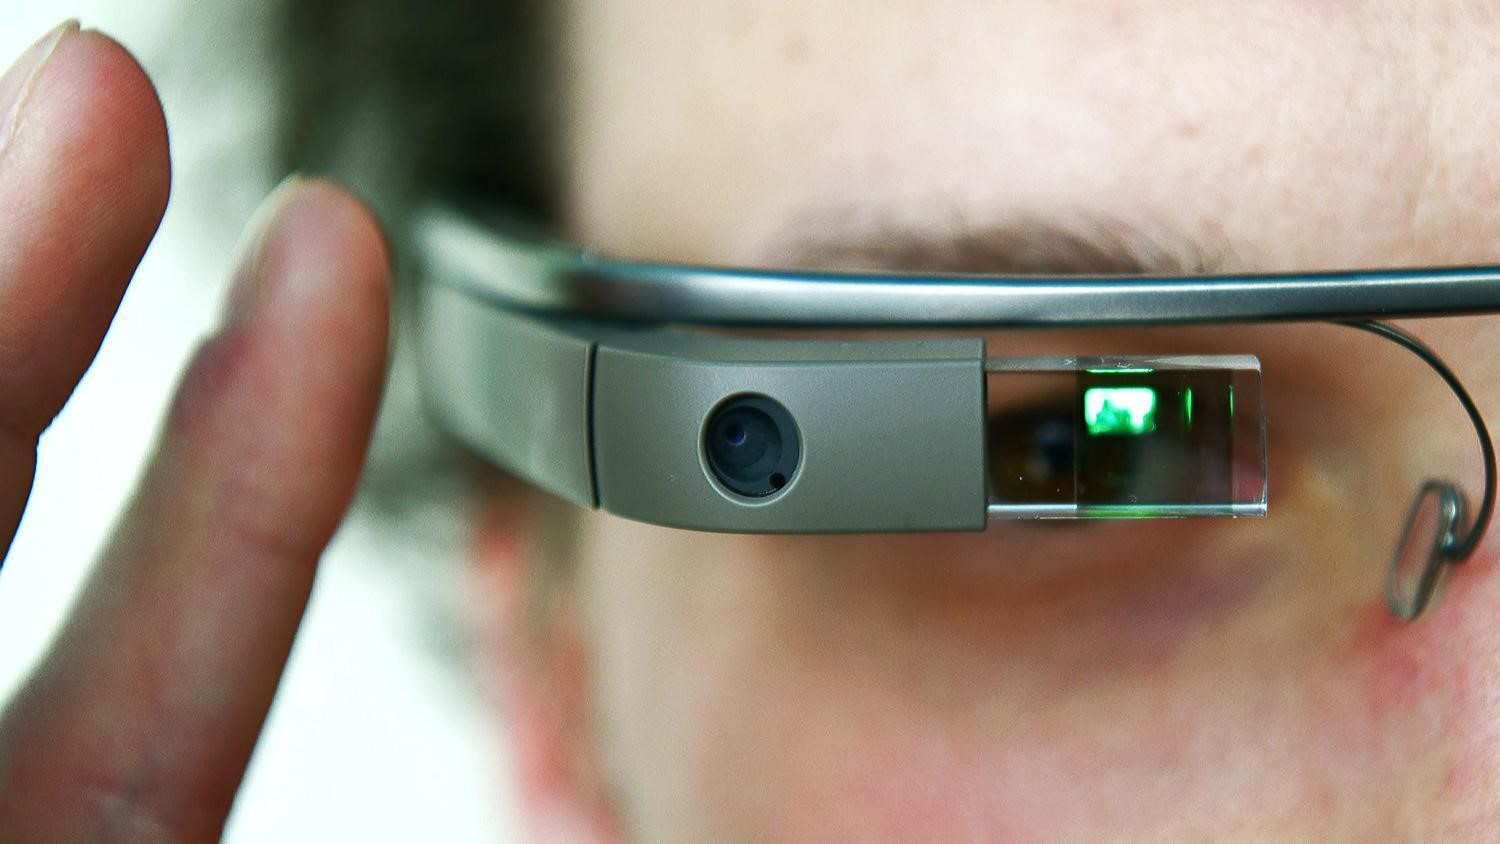
\includegraphics[width=240pt,height=180pt,keepaspectratio]{graphics/GoogleGlasses.jpg}
 \caption{\cite{glasses01}}
 \end{figure}
 \\
 \\
 Google Glass has 7 main functionalities\cite{functionsglasses}:
 \\
 \\
 The first one ,it doesn't need an extension of a smartphone or tablet. This gadget has it's own hardware such as in mobile phones. It can perform itself various day to day tasks, without moving the hands of a user. 
 \\
 \\
 The second function is , it can record a video or it will take picture, if the user just give an oral command. So in that case the user never have to touch a Button or the hardware. The photos and videos will be stored on the 4GB flash memory of the device and it can also be shared on social networking websites or emailed.
 \\
 \\
 The third function is , it shows the user text messages as well as emails that the user receives. Via voice commands the user can reply to the text message or email.
 \\
 \\
 The fourth function is about googling with this device. If the person like to find a lot of information , the user just have to ask a question and Google glass will pull the answer from the internet. For example ,the end-user can ask when the st. stephen's cathedral was built or to give a few pictures of the church. The answers or the pictures will be provide on the small screen in form of the users eye.
 \\
 \\
 The next feature is to show maps. Probably lots of people uses Google Maps, so Google Maps are integrated into Glass. The user will be able to chart the course of the journey or lookup locations. It is possible to do establishments via voice commands.
 \\
 \\
 The fifth feature is live video sharing. Google Glass has the ability to show the world what the user of the device sees  $\rightarrow$ live! A good example is , when the user is attending a family function such as the users child's school play or a concert, he/she can share the feed with her/his friends or family members in real-time. So he/she can make them a part of the experience.
 \\
 \\
 Google Glass's next features is , it has Google Now integrated. Google Now is a digital voice assistant. It will keep track of the daily habits , such as when the user leave for office and which  route the user takes.  Google Now  will give the user a alternate routes if there is a traffic on the way or it gives weather updates periodically and it has among various other functions.
 \\
 \\
 The last function from  Google Glass is translation from a language to another. The user have to ask Google Glass to translate a phrase or sentence from one language to another and it will speak that out.
 \\
 \\
 \begin{figure}[htbp]
 \centering
 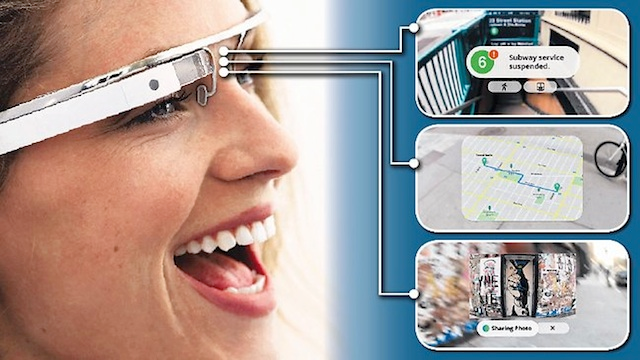
\includegraphics[width=240pt,height=180pt,keepaspectratio]{graphics/googlefunctions.png}
 \caption{\cite{glassesPic}}
 \end{figure}
 [7]
 \subsection{Usage of Augmented Reality}
 \subsubsection{Military and Law Enforcement }
 The military and law enforcement agencies uses  AR Technology for  full simulators which are designed to help in training.  For Example, a wide screen inside a room or a vehicle on which various scenarios is presented and the trainee must decide the best course of action.
 \\
 \\
 Some advanced Special Forces teams have basic AR goggles that, along with the land in sight, displays information such as altitude, angle of viewing, light intensity, and so on.AR technology also used by specialized night vision glasses. This device can display location and other information. The most of the unmanned vehicles in the military branches uses also AR technology as well. These vehicles, especially the aerial ones, can be thousands of kilometres away from their operators. The next point is that the vehicles have one or more cameras mounted on their exterior, which transmit video to their operator. This vehicle are equipped with several sensors as well. There is a sensor which sends data to the operator along with the video. This data is the processed and augmented over the video.  The operator's System with complex algorithms picks out the mark building or objects of interest. This kind of information will be displayed as an overlay on the video.\cite{AugmentedBook}
 \\
 \\
 \subsubsection{Vehicles}
 Nowadays AR technology started to be implemented in vehicles. Often there are multiple screens in the vehicle, each showing particular direction. So just think about there is only one screen and multiple cameras, the vehicle will either switch the feed automatically or have the option for the user to switch  between the cameras. The exterior of the vehicle has the ability to control the several cameras. The images from the camera will be shown on the screen and it is overlayed with useful data such as small map, compass, direction arrows, alternate routes, weather forecast and much more. This kind of technology is currently most visible in airplanes and trains at the moment. Some smart cars has the same ability ,but they are in test phase . The Submarines and ships are using this technology as well. The important thing is that Space Shuttles have this kind of AR technology also.
 \\
 \\
 It is possible to create apps which implement a sort of hybrid way on the Android platform. The reason is that the most Android devices seem to bee lacking in features that normal vehicles have, the same kind of features are not achieved. On the other hand, apps can be written for the help to navigate by using the GPS to get to the right location.  With the right API it is possible to write an APP to use the accelerometer to help with  acquiring the speed of the vehicle. Android device provides the AR power and the vehicle  provides the vehicle part.\cite{AugmentedBook}
 \\
 \\
 A example of a smart car:
 \begin{figure}[htbp]
 \centering
 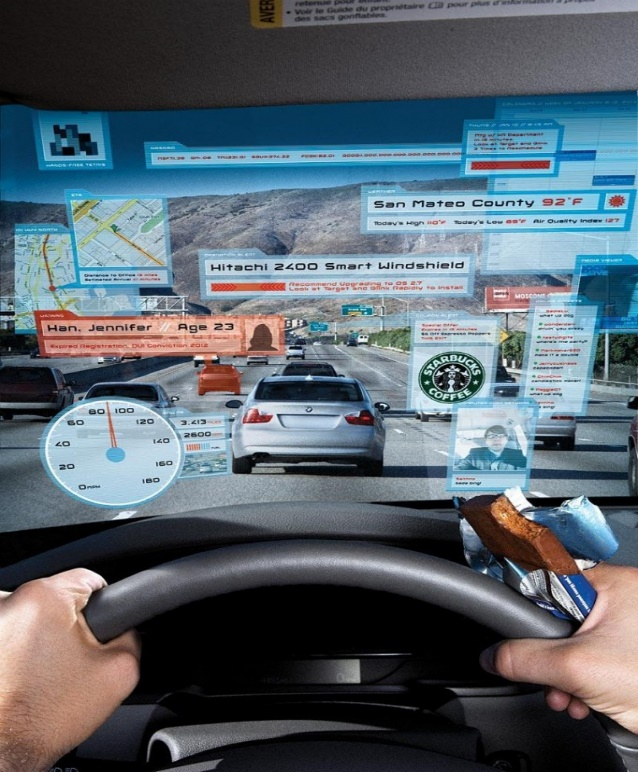
\includegraphics[width=240pt,height=180pt,keepaspectratio]{graphics/smartcar.png}
 \caption{\cite{smartcar}}
 \end{figure}
 [9]
 \subsubsection{Medical}
 AR technology is quite popular in the medical field.  This technology enables to become more common these days for surgeries.  With AR the error rate are smaller in Surgery branches. The reason is that the computer provides valuable inputs on the surgery and uses the information to control robots to perform some or all of the surgery.  Furthermore , the computer  can often provide alternative ways and instructions  on what can be done to improve the  surgery in real time.   Augmented Reality  stream , along with other data, has data which can be sent per remote to doctors, who can view the information of the patient as  if the patient were in front of them.
 \\
 \\
 In the medical field ,there are other medical apps of AR technology.  It is possible to use AR machines to monitor a large number of patients and make sure that their vital signs are under observation at all times.
 \\
 \\
 This kind of AR technology can never be implemented on a Android smartphone. The main reason is , it is to expensive.  To create such a app we need a team of very good developers, a team of highly skilled and experienced doctors and a large amount of money.\cite{AugmentedBook}
 \\
 \\
 \subsubsection{Trail Rooms}
 AR technology are widespread in several shops. The reason is , why some shops uses AR is to create a virtual trial room.  The idea of virtual trial room is  that the user stands in front of a screen with a camera mounted somewhere.  So the user will see himself displayed on the screen. The next point is the user uses an input devices such as a mouse or a keyboard to select any of the available clothing options. In the background the computer use a algorithm to augment that item onto the user's image and display it on the screen.  The  user can turn to view himself from all angles.\cite{AugmentedBook} 
 \\
 \\
 \subsubsection{Tourism}
 The Tourism branch is also using the AR technology.  Around the World, there are a lot of famous spots. So the organized tours now offer a head-mounted AR system that displays information about the current site and its buildings when the user look at it.  Furthermore the tourist can rebuild buildings, cities , landscapes and terrains as they existed in the past with the AR technology. The Tourism AR provide icons or markers for famous monuments. Tourism AR has the ability to find parks, restaurants, hotels and other tourist related sites and attractions in an unfamiliar city. These applications are not limited to historical places.\cite{AugmentedBook}
 \\
 \\
 \subsubsection{Architecture}
 In this world there a lot of camera-equipped machines that can generate a blueprint form an existing structure or display a virtual structure from the blueprints on the proceed site of constructions.  These functionality helps to design and check buildings. Augmented  reality technology provides the functionality to simulate natural disaster conditions. So it can show how the building structure will react under that kind of pressure.\cite{AugmentedBook}
 \\
 \\
 \subsubsection{Education}
 In Educational Institutes is AR technology very useful. Children or students can learn through AR. AR act in this field as  add-ons to the textbook material or as a virtual, 3d textbook in itself. Furthermore the AR give the ability for the student to \textit{relive} events as they are known to have happened, while never leaving their class.\cite{AugmentedBook}
 \\
 \\
 \subsubsection{Art}
 Augmented Reality helps  to create paintings, models and other forms of art.  The technology helps  to try out a particular design, before  actually putting it down in ink or craving it out of stone. It is also able to paint something virtually to see how they turn out and the artist can repaint as often he wants until he is satisfied . Then he can put it down on the canvas finally.\cite{AugmentedBook}
 \\
 \subsubsection{Translation}
 AR technology can be used for translate text from multiple languages all over the world. AR feature OCR and either have an entire cross-language dictionary on the device or it can translate the language over the Internet.    Few companies are producing apps with this ability. For this function we have to use  a ready-made optical character recognition(OCR) library to convert the images from the camera to text. The idea of OCR is it extract the text from image and put compare it with the translation dictionary or it can be translated through the internet. The translated result will be shown on the display.\cite{AugmentedBook}
 \\
 \subsubsection{Weather Forecasting}
 Most of the weather forecast app are augmented. The Data for the weather will be recorded and while the recording  the green backdrop serves as a  marker. If the recording is finished, a computer is used to add the map and position to match the forecaster's actions. AR  are used by transmitting the forecast live to the viewers .\cite{AugmentedBook}
 \\
 \\
 \subsection{Future of Augmented Reality}
 Augmented Reality is a growing up technology. It has amazing abilities, but few of them can't be implemented right now due to limitations in hardware and algorithms.\cite{AugmentedBook}
 \subsubsection{Virtual Experiences}
 
 
 
 In the future the AR technology could have a system ,which could transform from the current location into something completely different. A good example is , just imagine in the future you can live through movies by wearing  such a system and seeing the movie happen around. Probably this technology could convert the house of a user into a medieval castle or into the international space station. Furthermore with the combination  of smell-emitting technology and the aural AR , it could make the environment lifelike and  feel completely real. In addition to this ,it is capable to add a emulation of the sense of touch with a body suit. That will make it absolutely and undeniably real. \cite{AugmentedBook}
 \\
 \\
 \subsubsection{Holograms}
 The following point is that AR allows  the user to have a live direct or indirect of the world. That could enable users to have holograms in front of them. These holograms could be interactive or merely descriptive.  For instance somebody is calling you and a hologram of these person appears in front of you. So we see AR could have this ability.\cite{AugmentedBook}
 \subsubsection{Video Conferencing}
 In the future , multiple people will appear in the same conference room if a video feed of a conference room is  transmitted to them with the AR technology.  The idea is that the people could use  the webcam to \textit{appear} in the seat of the room, along with the members.\cite{AugmentedBook}
 \\
 \\
 This idea could probably help people who are not able to attend the meeting ,because they are thousands of kilometres away. So this futuristic Video Conferencing could solve this problem. Furthermore for this implementation we need a high-speed internet and the person which participating the conference have to stay  exactly in the same place, if not then the algorithm have to positioning him again and these need a big amount of data streaming.\cite{AugmentedBook}
 \\
 \\
 \subsubsection{Movies}
 This technology can be used  to play entire movies.  The idea is that the theatre could be replaced with the background of the movie  or the theatre could be replaced with the actors only.  The first method is that the actors could be augmented onto the background and in  other way the background could be augmented behind the actors. The second method would reduce the costs of the shooting. These methods could provide more realistic and fun movies.\cite{AugmentedBook}
 \\
 \\
 \subsubsection{Gesture Control}
 AR could be used for many gesture controls such as eye dialing.   It should track the eye movement from the user and should select the right the appropriate number key. If the key has been selected , the user could blink to press that number and then proceed to select the next key. This kind of algorithm could be implemented to control music players, mobile apps, computers and other form of technology.\cite{AugmentedBook}
 \\
 \\
 To create app with this algorithm requires a few things:
 \\
 \\
 First of all it needs a front camera with a reasonable resolution. The second thing is that the algorithm has to be well written to detect fine eye movements  and to convert it to the right information. This algorithm has to filter other movements.
 \\
 \\
 \subsection{Summary}
 So we see that AR is a developing technology. The basic requirements for the technology is back and front camera , GPS, accelerometer and compass. Most of the requirements are fulfilled by almost all Android devices on the market. Now it is great time to create AR apps, because in these the competition is very low and it is good to start business with it. Augmented Reality are quite popular in many fields such as Military, Medical and Education.
 \\
 \\
 \begin{figure}[H]
 \centering
 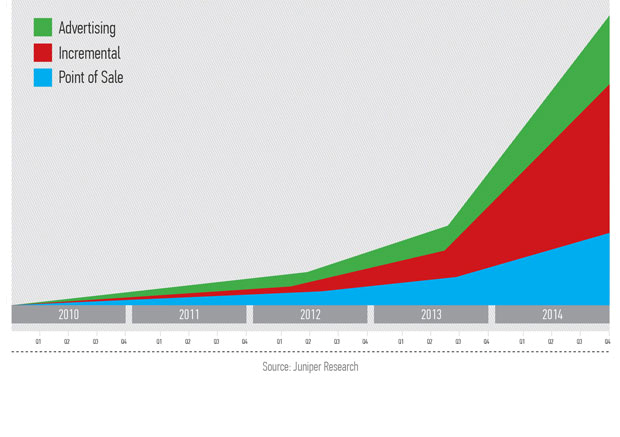
\includegraphics[width=240pt,height=180pt,keepaspectratio]{graphics/statistics.png}
 \caption{\cite{statistics}}
 \end{figure}
 [11]
 \\
 The Graph is showing the Advertising and Point of Sale rate of AR. We can see the graph is increasing year to year. The Result of the Graph is that the features of the technology is increasing.
